


Sovelluksessa on ominaisuus, missä käyttäjät voivat seurata treenikertojen määrää ja edistymistä.
Tiedot käyttäjä datasta on tallennettu tietokantaan mutta niistä pitäisi saada asiakkaalle raportti.
Asiakkaan pitäisi pystyä käyttöliittymästä valitsemaan millaisen raportin hän haluaa ja mitä tietoja raporttiin laitetaan.
Tämä vaatii kommunikaatiota clientin, palvelimen ja tietokannan välillä. 
\medskip

\subsection*{Meteor}


%Meteor on, mongoDB tietokantaa lukuunottamatta, avoimeen lähdekoodiin perustuva full-stack web-framework. 
Meteor on avoimeen lähdekoodiin perustuva full-stack web-framwork, mongodb tietokantaa lukuunottamatta, jonka meteor paketoi mukanaan.
Meteorilla on integraatio moneen yleiseen frontend-framework:kiin, kuten vue, react, svelte tai angular.
\medskip




Meteor antaa monta työkalua clientin, palvelimen ja tietokannan väliselle kommunikaatiolle, kuten metodit ja subscriber-publisher malli.
Meteor methodit antaa mahdollisuuden luoda rajapinnan palvelimen ja clientin väliselle kommunikaatiolle ja 
subscriber-publisher auttaa käyttöliittymän päivittämisessä tietokannan muututtua.





\medskip




%https://www.leviathansecurity.com/blog/websockets-and-meteor-a-penetration-testers-guide-to-meteor



\subsection*{Subscriber publisher}

Yleinen ongelma Web-sovelluksissa on käyttöliittymän päivitys, kun palvelimella tai tietokannassa tapahtuu muutoksia. 
Nettisivuilla, jotka käyttävät RESTful rajapintoja, lähetettäisi get request palvelimelle, kun halutaan pyytää tietokannasta dataa. Client ei tietäisi jos data on vanhaa tai jos se on päivittynyt palvelimella.
Restful rajapinnallisissa sivustoissa pitäisi yhdistää palvelin ja client esimerkiksi web-socketilla, jolloin palvelin voi ilmoittaa että on tullut muutos dataan.

\medskip

Meteor käyttää subscriber-publisher mallia, jossa client on yhdistetty palvelimeen web-socketin kautta. 
%
Palvelin voi julkaista osia tietokannasta meteor.publish-funktiolla ja asiakas voi tilata ne. Jos asiakas tilaa tämän julkaisun, se saa ilmoituksen aina, kun tiedot, jotka asiakas on tilannut, muuttuvat.
Tällä tavalla tiedetään mitä tietoa client haluaa ja mitkä osat päivittyy, joten palvelimen ei tarvitse lähettää kaikkea tietokanta muutoksia clientille, vaan ne mitkä client on tilannut.
Meteor voi sitten päivittää käyttöliittymän osia, jotka ovat riippuvaisia kyseisistä tiedoista. 

% kuvia vaikka publish ja subscribe kutsuista
% esimerkki kuva publishista mongodb käytössä
%esimerkki client subscirbestä 
%https://docs.meteor.com/api/pubsub#Meteor-subscribe
%tästä tehdään esimerkki koodi ja siitä screenshot
% kuva on hyvä jos  muutetaan raporttinluonti omalle viikolle


\medskip

Meteor päivittää komponentit mitkä ovat riippuvaisia halutusta datasta automaattisesti. Tekien käyttöliittymä koodista puhtampaa.


\medskip



\subsection*{Methodit}

Meteor ei käytä RESTful rajapintaa palvelimen ja clientin välillä, vain Meteorin methodeja.
Methodit suoritetaan ja määritetään funktioina palvelimen puolella, ja niitä voi kutsua clientistä tai palvelimelta.
Metodit antavat kutsujasta tietoa, esim onko kutsuja kirjautunut sisään ja jos on niin mikä on hänen käyttäjätunnus. 
Näin voi helposti katsoa onko kutsujalla tai käyttäjällä oikeuksia metodin kutsumiseen.
\medskip


% kuva methodi määritelmästä ja seloitus mitä tapahtuu

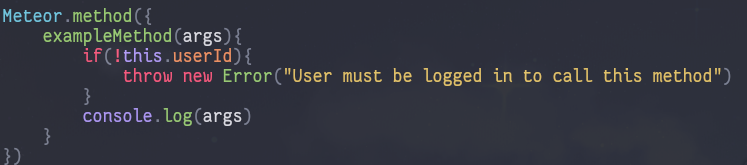
\includegraphics[width=15cm]{src/public/methodexample.png}\\
Meteor methodin määritelmä
\medskip

Muvassa on meteor methodin määritelmä. "exampleMethod"{} methodi katsoo onko kutsuja kirjautunut sisään, jos käyttäjä ei ole kirjautunut niin heitetään error.
Jos käyttäjä on kirjautunut sisään tulostetaan argumentit. Argumentit tulostetaan palvelimelle.  





\subsection*{Raportin luonti}

%selostus raportin specista ja mitä sen pitää tehdä

Raporttiluonti ominausuuden määritelmänä oli, saada ulos exelissä avattava tiedosto, jossa näkyisi käyttäjän nimi, treenikertojen määrä ja progressio ominaisuuden ensimmäinen ja viimeinen arvo.
Raportin luonti pitää olla laajennettava. Raportissa olevan datan formaatti ja ulostulevan tiedosto formaatin pitää olla muutettavissa.
\medskip


% selostus miten raportti toimii käytännössä. kirjoita kirjakielellä

Raportin luonti toimii käytännössä näin.
Client kutsuu getReportData methodia ja antaa sille objektin argumenttina, jossa on tietoa mitä dataa halutaan lisätä raporttiin ja missä muodossa.
Methodi varmistaa onko kutsuja kirjautunut sisään, ja onko hänellä tarvittavat oikeudet suorittaa methodi.
Palvelin käy läpi asetukset mitä raporttiin halutaan ja lähettää datan takaisin clientille, josta client muodostaa tiedoston.
\medskip

% selitys siitä miksi tiedosto tehdään clientillä

Tiedosto luodaan clientillä eikä palvelimella, koska jos sen tekisi normaalisti palvelimella se on estävä funktio,
jolloin palvelin voisi jäätyä silloin kun tehdään isoa dokumentti, ja 
vaikka tiedoston tekemisen voi tehdä asynkrooniseksi se silti hidastaisi palvelinta. 
%teknisesti väärää tietoa ei tule ylimääräisiä kustannuksia sillä heroku veroittaa tunnilta. 
Kun client tekee tiedostoon työn niin vältetään ylimääräisiltä palvelin kustannuksilla.
Tiedoston valmistuttua käyttäjä voi ladata sen.
\medskip


\subsection*{Yhteenveto}

Meteor on suunniteltu nopeaan kehitykseen ja se näkyy sub-pub mallissa ja metodeissa.
Kun käyttää sub-pub niin kehittäjän ei tarvitse kirjoittaa käyttöliittymä koodiin logiikkaa sen päivittämiselle, vaan meteor hoitaa sen automaattisesti.
Methodit on nopea tapa tehdä rajapinta ja se on helposti yksikkö testattavissa. metodit myös luo helpon tavan tietää onko kutsujalla oikeuksia metodiin, joka luo lisä turvallisuutta.
\medskip

% kirjota hyvin
Raportin luonti ominaisuus toimii määritelmien mukaan.
%
Uusien tiedosto -formaattien tai -ulkoasujen lisääminen on helppoa. 
Tiedoston luonti tehdään clientillä, joten uuden tiedostoformaatin lisääminen edeltää funktion lisäämistä, 
joka ottaa argumenttina datan ja palauttaa halutun tiedoston blob:ina (binary large object).
%
Metodille annetaan objekti jossa kerrotaan mitä dataa halutaan, joten eri datan saanti palvelimelta edeltää vain objektin muuttamista.





